%
%
%
\long\def\comment#1{}
\newif\ifcover

% パタンはtt
% 出力文字列はsf

\documentclass{article}
\usepackage{times}
\usepackage{uist04}

\usepackage{here} % [H]とするとその場所に配置されるらしい

% \def\up{ 
\includegraphics[width=3mm,bb=0 0 36 36]{figures/uptriangle.pdf} }
% \def\down{ 
\includegraphics[width=3mm,bb=0 0 36 36]{figures/downtriangle.pdf} }
% \def\right{ 
\includegraphics[width=3mm,bb=0 0 36 36]{figures/righttriangle.pdf} }
% \def\left{ 
\includegraphics[width=3mm,bb=0 0 36 36]{figures/lefttriangle.pdf} }
\def\up{▲}
\def\down{▼}
\def\right{▶}
\def\left{◀}

\long\def\ttt#1{\texttt{\small #1}}
\long\def\tsf#1{\textsf{\small{#1}}}
\long\def\tit#1{\textit{\small{#1}}}

% \long\def\ST{\textsf{\small{Strotor}}}
\long\def\U{\textsf{\small{U}}}
\long\def\D{\textsf{\small{D}}}

\def\SC{\textsf{\small Serencast}}
\def\SB{\textsf{\small Scrapbox}}

\usepackage{graphicx}
% mediabb.sty というのを使うとPDFをそのままincludegraphicsできるらしい。
% http://www.ns.musashi-tech.ac.jp/~inoue/Pages/TeX/mediabb.sty.html
%
% \usepackage{mediabb}
% \usepackage{ascmac}

\begin{document}
\title{Non-click browsing}
\author{
\begin{tabular}{l}
\parbox{5.5cm}{
\begin{center}
% Toshiyuki Masui\\
% Keio University\\
% masui@pitecan.com
~ \\
~ \\
~
\end{center}
}
\end{tabular}
}
\maketitle
\abstract

We introduce a novel simple interaction technique for finding and browsing
data in a huge hierarchical database using only two keys or
one rotating device.
% that can generate two different signals based on the rotation direction.

We can enjoy various kinds of movies, musics, books,
etc. distribued from many service providers like Amazon and Netflix.
However, 
finding a data from the huge database is not a trivial task. Users can
either find an entry using keywords, or using a menu based
on a hierarchical structure of the database.
After successfully finding a candidate data,
the user should confirm that he wants to watch it by pressing a ``select'' button.
If the user finds that the data is not the one he wanted,
he should go back to the previous state and perform the search again.

In the past, when only a small number of ``channels'' were availale
from broadcast TV stations, the only thing users could do was
using the ``television dial'' to select a ``channel'' and watch the
broadcasted data.
Although the number of the sources were limited,
the user interface for selecting a station was simple.
%
We introduce a simple interaction technique called ``Gear'',
with which users can select an entry from a very large hiearchial database and
browse it instantly, just like we could select a channel and enjoy a TV program
using old television dials.

\keywords Input device, Information navigation, Hierarchical data, Gear, Serencast

\tolerance=400 
  % makes some lines with lots of white space, but 	
  % tends to prevent words from sticking out in the margin

\section*{INTRODUCTION}

Large data are often represented as a hierarchical structure, and
various navigation methods are provided for exploring the data.
For example, files on Unix are structured hierarchically, and
many commands (\tsf{cd}, \tsf{ls}, etc.) and APIs are provided for exploring the file system.
Large dictionary database can also be treated as a large
hierarchical data, since the name of the entry can be treated hierarchically:
e.g. an entry for ``\tsf{dictionary}'' can be stored under ``\tsf{d}'', ``\tsf{d/i}'', and so on.

Many information visualization techniques and navigation techniques
have been proposed for handling large hierarchical data.
On modern personal computers,
multiple GUI techniques are provided for
exploring the hierarchical file structure, because
there is no best interaction technique that fits to all the users and situations.
On MacOS, four GUI methods are provided for browsing the file system.

% there is no single interaction technique that is always good for any situation.
% ZUIの話, ハイパーリンクでたどる方法もある

When a user cannot use GUI,
selection-based interaction techniques are used for
finding information in hierarchical data.
For example, a user can hierarchically find a music data by
selecting an artist from the list of artist names,
selecting an album title from the title list,
and selecting a music data from the song list.
% Users can do the selection jobs either by using a mouse or by using arrow keys.
% For exaple,
Users can use two keys for choosing an entry from the list
(e.g. selecting an artist from the artist list),
and use another key for selecting an entry and moving to the next level
(e.g. selecting an artist and show album titles).
It is also necessary to provide a way to go back to the previous state, and
yet another key can be used for that task
(e.g. showing the artist list for artist selection).
This 4-way navigation is popular on small mp3 players\footnote{
  e.g. \textsf{http://www.iriver.com/product/view.asp?pCode=003\&pNo=37}
} and remote controllers like AppleRemote\footnote{\textsf{http://en.wikipedia.org/wiki/Apple\_Remote}}
for selecting a song from the hierarchical data.
4-way navigation is also available on desktop software like Finder.app on Mac.

% Amazon FireTV

\begin{figure}[H]
\centerline{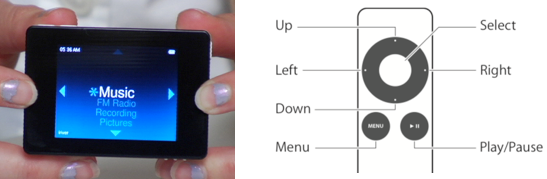
\includegraphics[width=80mm,bb=0 0 547 179]{figures/4buttons.png}}
\caption{4-button controllers on a small mp3 player (left) and AppleRemote (right).}
\label{u10}
\end{figure}

% http://www.reigncom.com/eng/media/press/en_pr_read.asp?no_noti=1630&cd_noti_host=9
% D-Click Control System

% Small devices like Rio MP3 player and remote controllers like AppleRemote have
% 4 buttons for selecting a song from the hierarchical data.

Using 4 keys might be okay on these devices, but it would be much better
if we could perform the navigation task using simpler dvices that have only 2 keys.
In that case, we can also use a rotating device like a disk or a wheel for the navigation,
since such devices can generate 2 signals based on the rotation direction (Figure \ref{rotation}).
%
% We have developed a new navigation technique where only two keys are required
% for exploring large hierarchical data, and implemented the system on
% a rotating device ``Strotor''.
%
We have developed a new navigation technique called ``{Gear}'',
where users can explore a large hierarchical database by simple rotating operations.

\begin{figure}[H]
\centerline{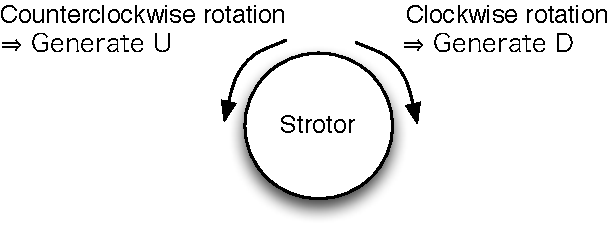
\includegraphics[width=60mm,bb=0 0 294 110]{figures/rotation.pdf}}
\caption{Using a rotation device for generating key events.}
\label{rotation}
\end{figure}

\section*{NAVIGATION METHOD AND EXAMPLES}
\label{navigation}

Interaction with Gear is based on the following simple principles.
Two types of operations, ``{\up}'' (up) and ``{\down}'' (down), are used for the navigation.
They can be performed either by rotating the Gear device or pressing keys.

\begin{enumerate}
\item A portion of the hierarchical data is shown to the user as a list.

\item One element in the list is selected and highlighted.

% \item Display the selected element, its siblings, its ancestors and their siblings.

\item When an elemente is selected, its siblings, its ancestors and their siblings are displayed
around the selected element.

\item Users can issue {\up} to select the element above the currently selected element,
or issue {\down} to select the element below the selected element.
Whenever the selection is changed, 3. is performed.
If the depth of the newly selected element is different from the currently
selected element, siblings of the currently selected element disappear.

\item When a newly selected element has children and the user performs no further action,
the first child of the selected elemente is newly selected, and 3. is performed.
As a result, all the siblings of the newly selected element
(the first child of the currently selected element) appear in the list.

\end{enumerate}

We show how Gear works, using a hierarchical data structure of
a shops list in a shopping mall shown in Figure \ref{fig1} as example data.
A rectangles with a thick border represent shop categories, and
other rectangles represent individual shops.

\begin{figure}[H]
% 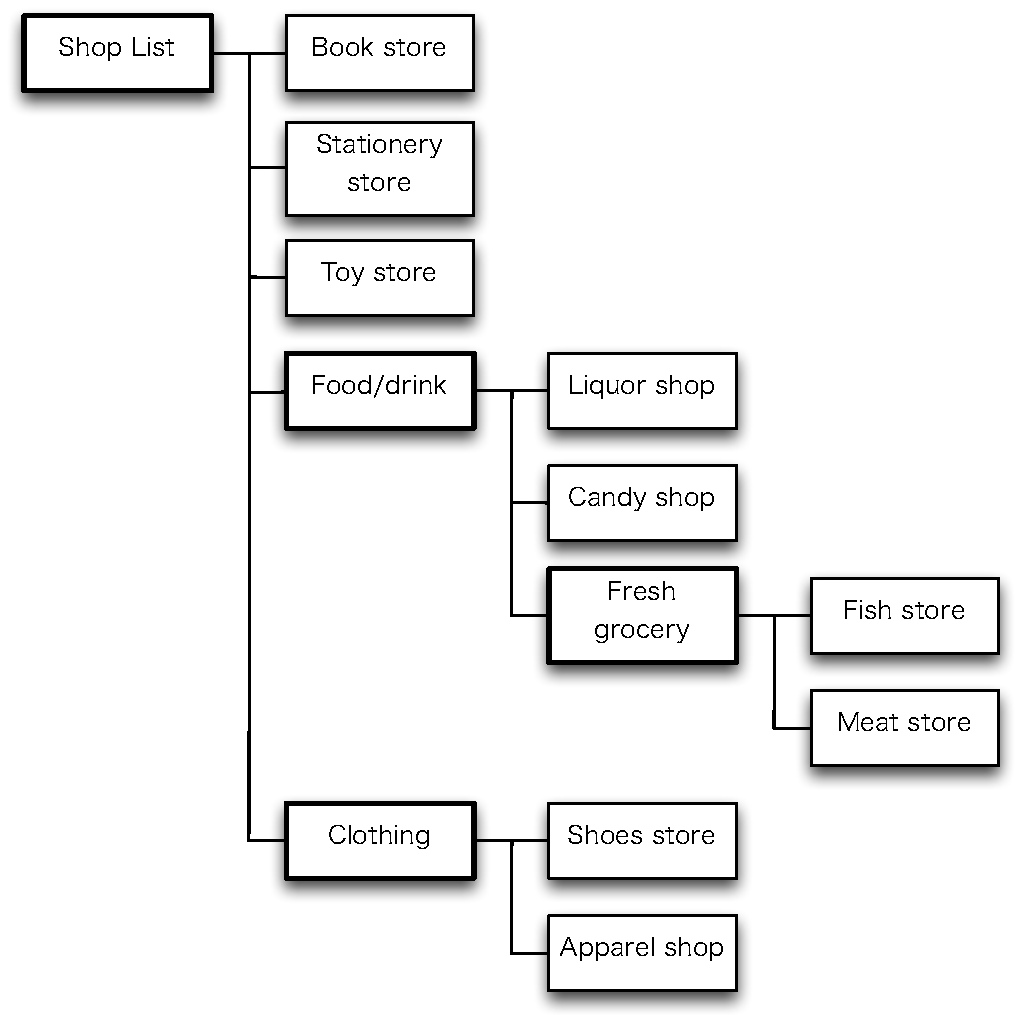
\includegraphics[width=70mm]{figures/fig1.pdf}
\centerline{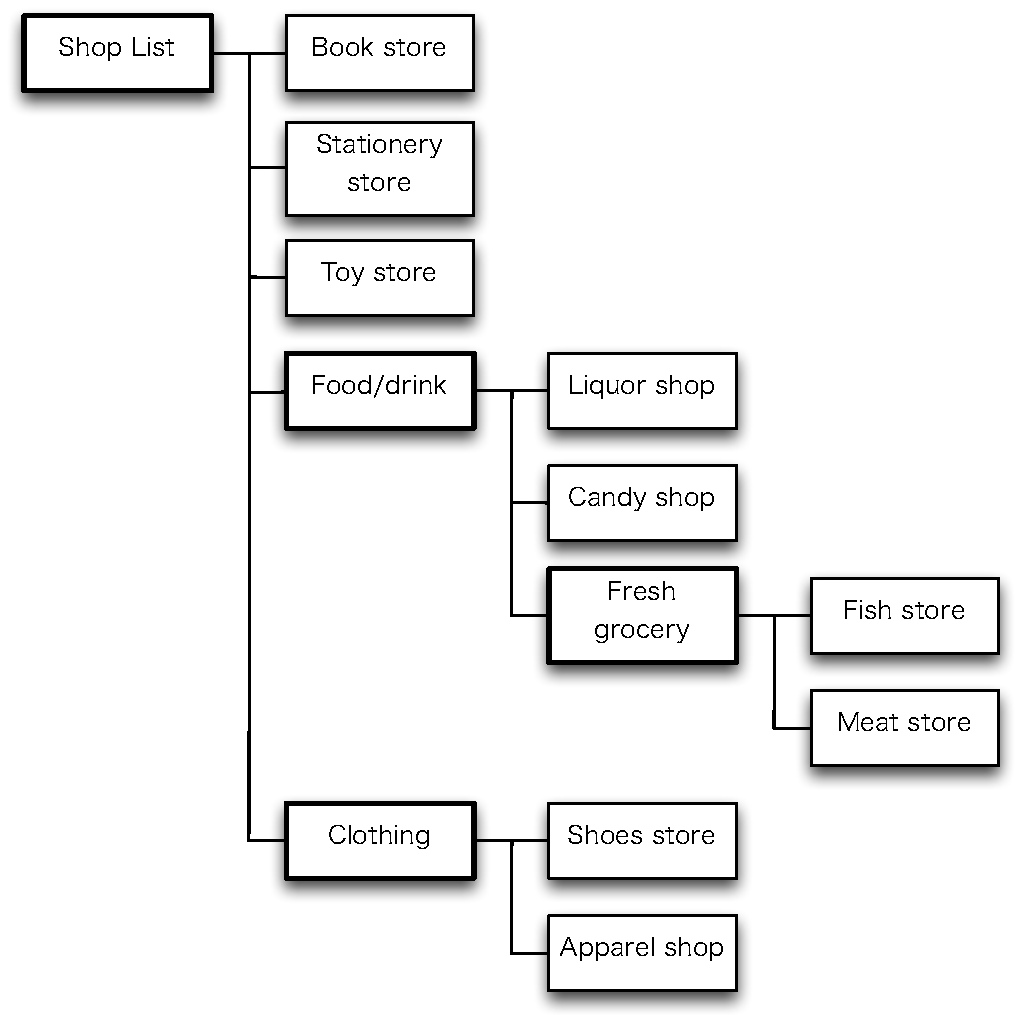
\includegraphics[width=80mm,bb=0 0 490 490]{figures/fig1.pdf}}
\caption{Sample data: shops in a shopping mall.}
\label{fig1}
\end{figure}

When a user starts the exploration, only the shops and categories
at the top level are displayed (Figure \ref{fig2}).
When the user issues {\down},
the second element (\tsf{Stationery store}) is selected (Figure \ref{fig3}).

\def\menuwidth{22mm}

\begin{figure}[H]
\centerline{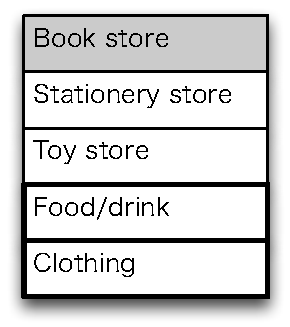
\includegraphics[width=\menuwidth, bb=0 0 139 157]{figures/fig2.pdf}}
\caption{Initial display.}
\label{fig2}
\end{figure}

\begin{figure}[H]
\centerline{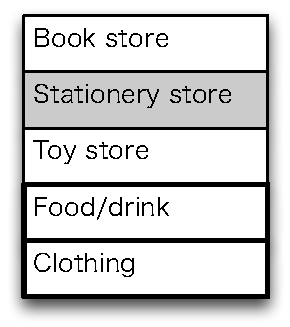
\includegraphics[width=\menuwidth,bb=0 0 139 157]{figures/fig3.pdf}}
\caption{Typing {\down}.}
\label{fig3}
\end{figure}

If the user issues {\down} two more times, 
\tsf{Food/drink} category is selected (Figure \ref{fig4}).
If the user stops the operation and waits for a moment, the shops under the \tsf{Food/drink}
category are automatically displayed,
and the first entry (\tsf{Liquor shop}) is selected (Figure \ref{fig5}).

\begin{figure}[H]
\centerline{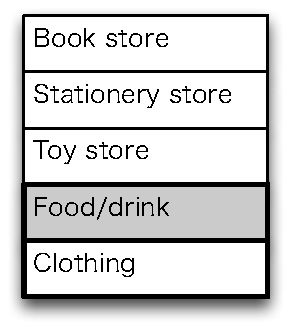
\includegraphics[width=\menuwidth,bb=0 0 139 157]{figures/fig4.pdf}}
\caption{Selecting Food/drink.}
\label{fig4}
\end{figure}

\begin{figure}[H]
\centerline{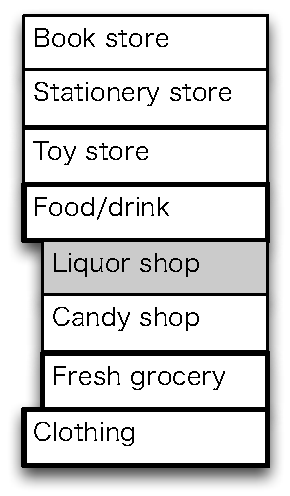
\includegraphics[width=\menuwidth,bb=0 0 139 238]{figures/fig5.pdf}}
\caption{Selecting Liquor shop.}
\label{fig5}
\end{figure}

When the user issues {\down} twice here,
\tsf{Fresh grocery} category is selected (Figure \ref{fig6}).

\begin{figure}[H]
\centerline{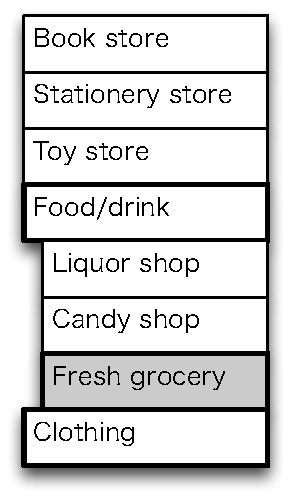
\includegraphics[width=\menuwidth,bb=0 0 139 238]{figures/fig6.pdf}}
\caption{Selecting Fresh grocery.}
\label{fig6}
\end{figure}

If the user keeps issuing {\down}, 
the list will change to Figure \ref{fig8},
without expanding the children of \tsf{Fresh grocery}.

\begin{figure}[H]
\centerline{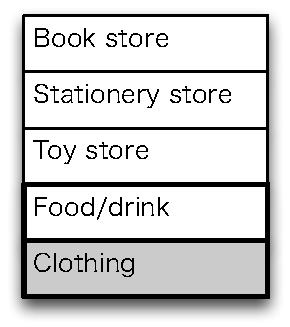
\includegraphics[width=\menuwidth,bb=0 0 139 157]{figures/fig8.pdf}}
\caption{Selecting Clothing.}
\label{fig8}
\end{figure}

If the use stops issuing {\down} at Figure \ref{fig6},
the shops under category \tsf{Fresh grocery} is automatically selected (Figure \ref{fig7}).

\begin{figure}[H]
\centerline{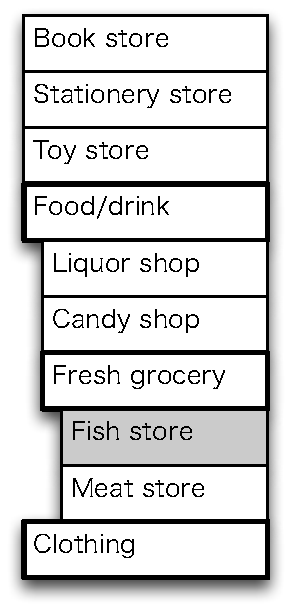
\includegraphics[width=\menuwidth,bb=0 0 139 292]{figures/fig7.pdf}}
\caption{Selecting Fish store.}
\label{fig7}
\end{figure}

When the user issues {\up} here, \tsf{Fresh grocery} is selected,
and the shops under \tsf{Fresh grocery} disappears, 
resulting in the same state as Figure \ref{fig6}.
If the user issues {\up} two more times, the display changes to the state
shown in Figure \ref{fig5},
and one more {\up} will set the system to the state of Figure \ref{fig4}.

If the user issues {\down} in Figure \ref{fig4}, the next visible entry
(\tsf{Clothing}) is selected (Figure \ref{fig8}), and then the state changes to Figure \ref{fig9}.

\begin{figure}[H]
\centerline{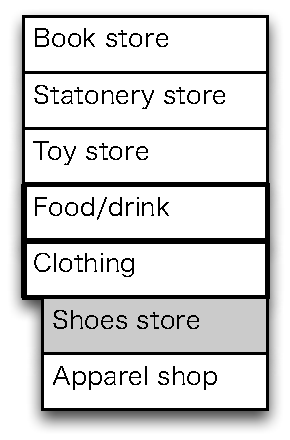
\includegraphics[width=\menuwidth,bb=0 0 139 211]{figures/fig9.pdf}}
\caption{Selecting Shoes store.}
\label{fig9}
\end{figure}

When the user issues {\down} twice in Figure \ref{fig7},
\tsf{Clothing} is selected, and the category under \tsf{Food/drink} will shrinke (Figure \ref{fig8}).

In this way, users can explore the hierarchical structure
only by issuing {\up} and {\down} at the right timing.

\section{SERENCAST: A NON-CLICK BROWSING SERVICE}

% SerencastというサービスでGearを使う
% SerencastはScrapboxを利用したものである

To prove that Gear is useful for selecting an entry from a very
large hierarchical database,
we have developed the ``\tsf{Serencast.com}'' service, where
users can enjoy movies, musics, and other Web services
on the browser with the Gear interface.
{\SC} is implemented in JavaScript, and runs on modern browsers 

{\SC} uses the ``\tsf{Scrapbox.io}'' wiki service\footnote{
  \tsf{https://Scrapbox.io/}
} for listing the contents of the hierarchical database.
{\SB} is an interactive wiki\footnote{
  \tsf{https://en.wikipedia.org/wiki/Wiki}
} system where users can share and edit texts on the Web browser.
A user can create a {\SB} ``project'', and create pages
that consists of texts and links,
and people can share the page and edit it freely on their browsers.

\begin{figure}[H]
\centerline{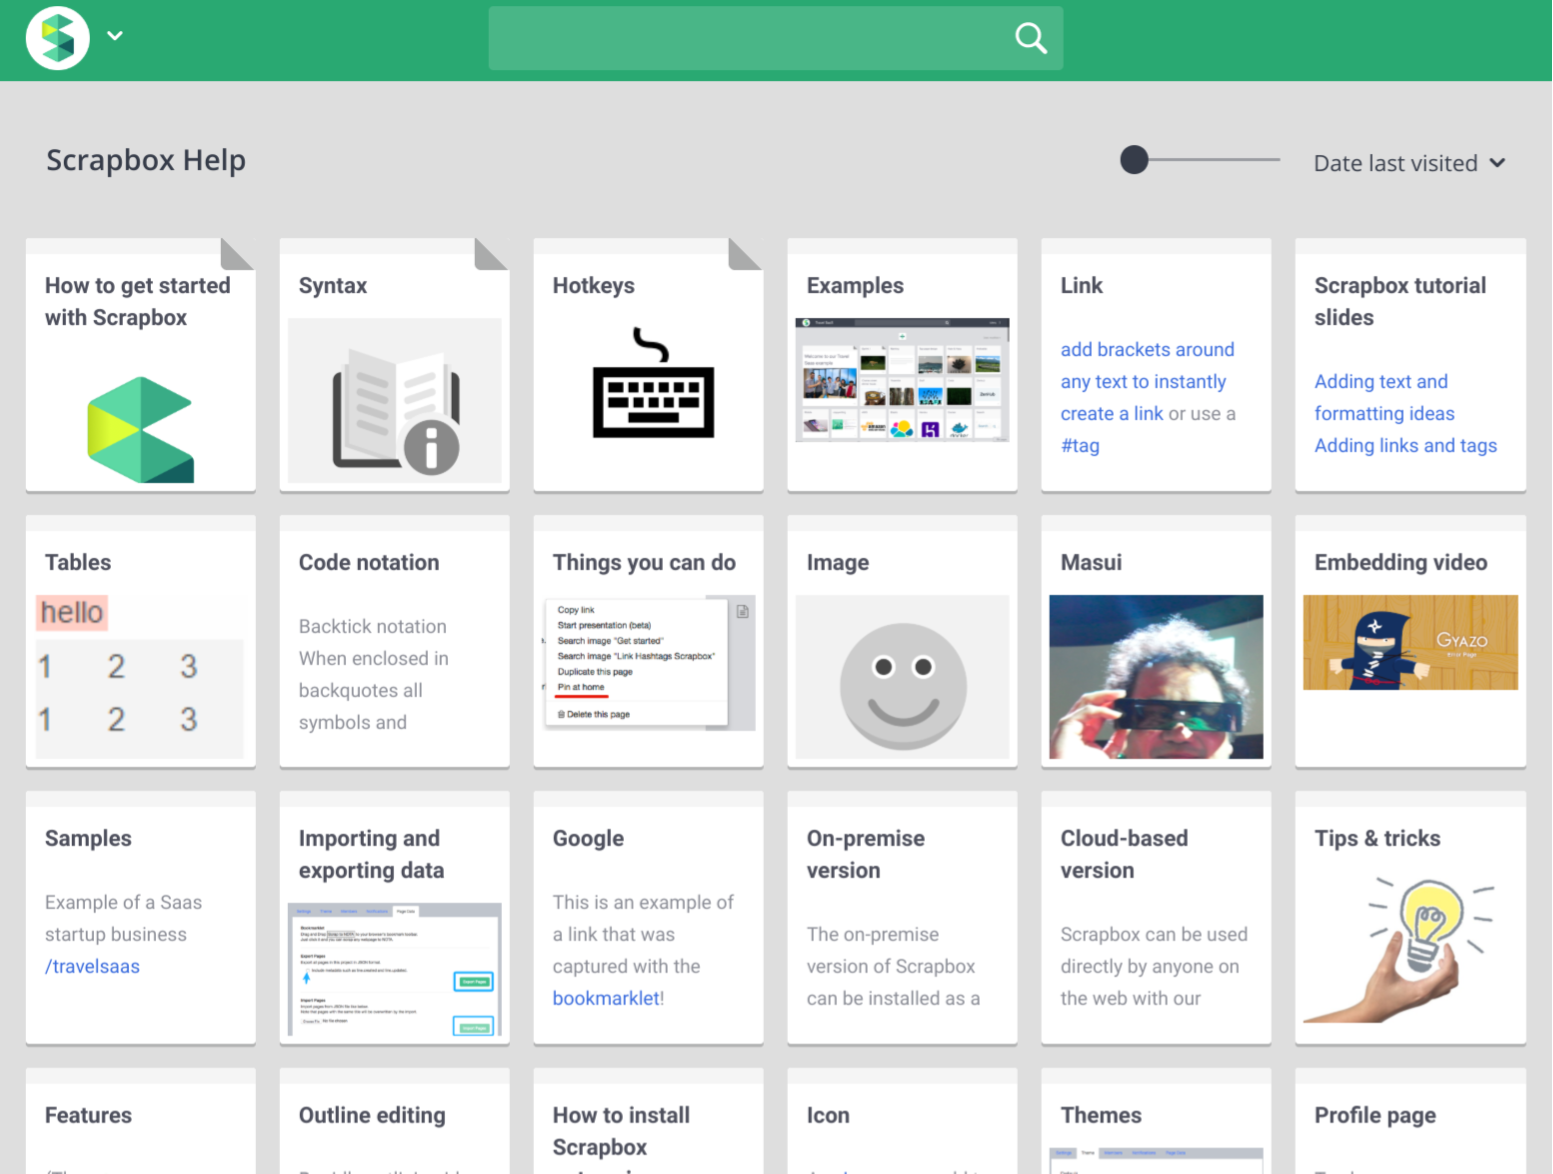
\includegraphics[width=80mm,bb=0 0 1553 1174]{figures/28818d749896f87f3eb8bd6b6f9e9a36.png}}
\caption{An example of a {\SB} project.}
\label{exampleproject}
\end{figure}

Figure \ref{exampleproject} shows an example of a {\SB} project.
The title of the project is ``Scrapbox help'', and
many pages like ``Features'' exist inthe project.

\begin{figure}[H]
\centerline{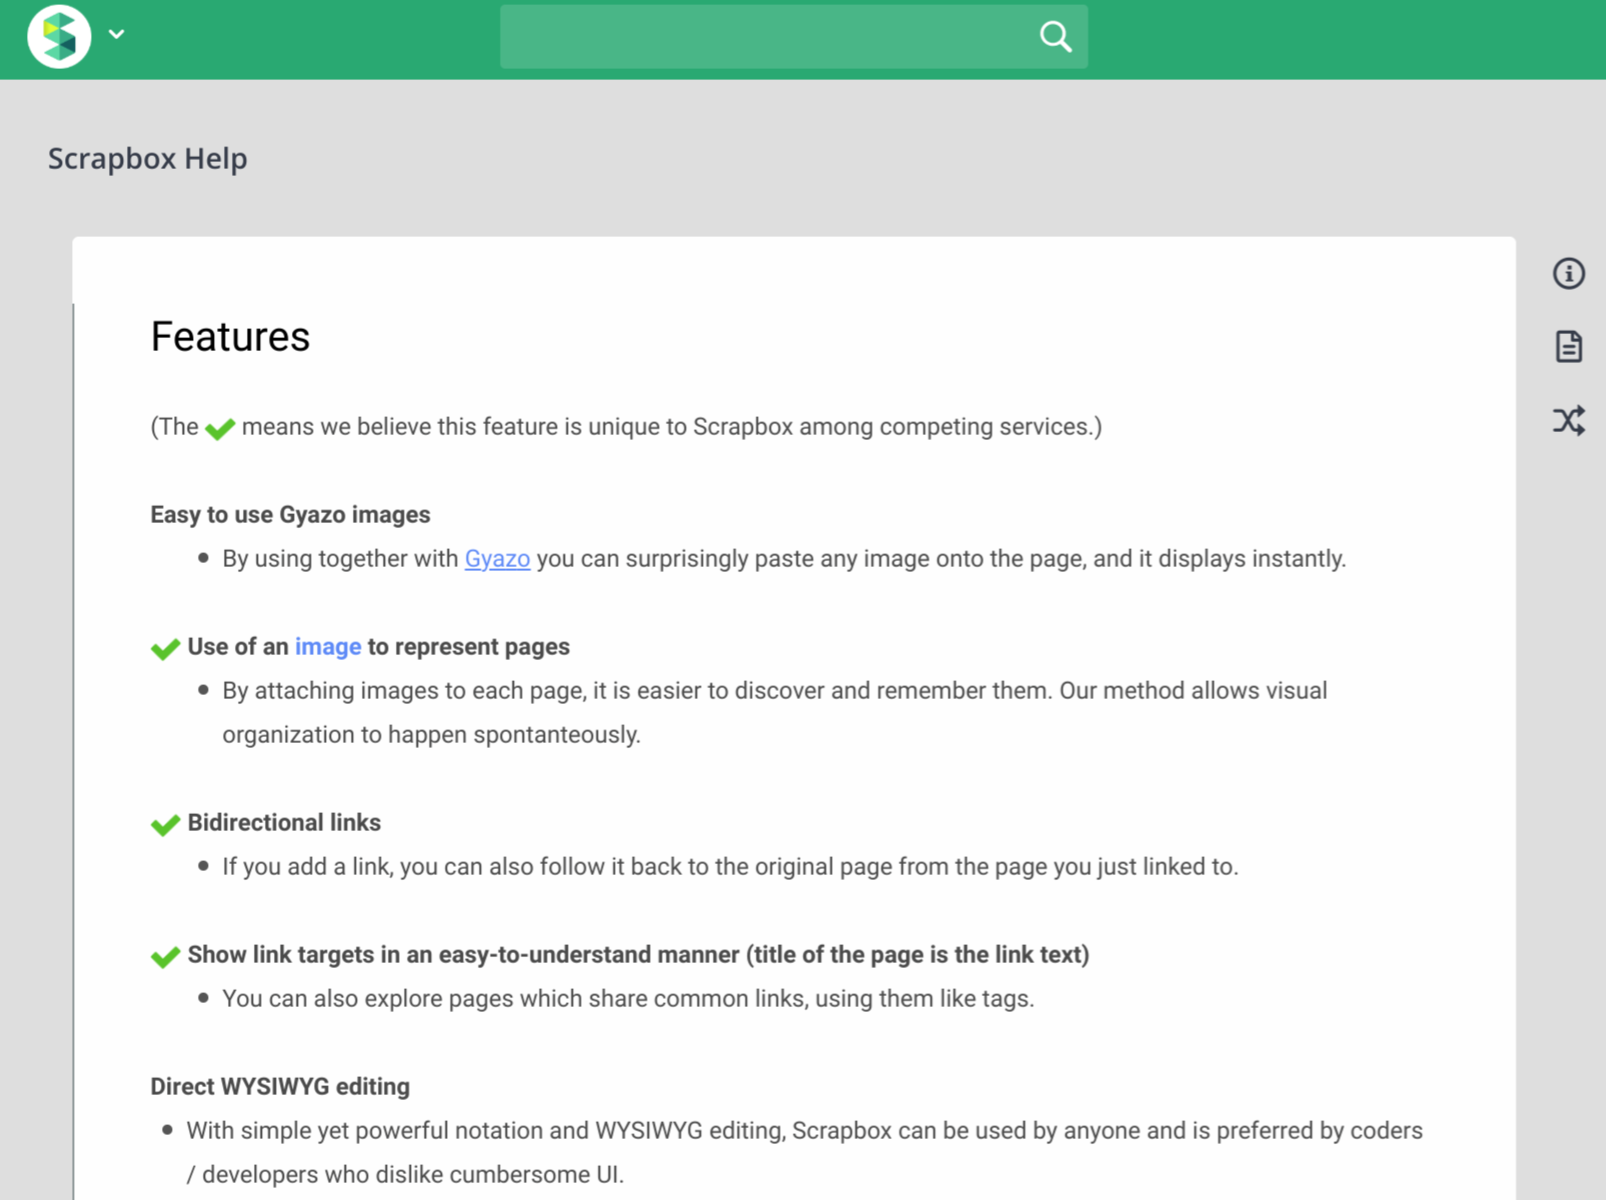
\includegraphics[width=80mm,bb=0 0 1606 1200]{figures/9e867c325bafc415bd0870c1717fbaf7.png}}
\caption{An example {\SB} page.}
\label{examplepage}
\end{figure}

Figure \ref{examplepage} is an example of a {\SB} page.
%
The page is based on plain text just like an WikiPedia page is based on plain text.
Users can use special markup tags
like ``\texttt{[}'' and ``\texttt{]}'' to show bold texts, icons, URL links,
and links to other pages.
In this example, a URL link to {\tsf{http://gyazo.com}} is used
just like \tsf{A} tags used in HTML.

The raw text of the {\SB} page looks like this:

{\scriptsize
\begin{verbatim}
Features
(The [Check.icon] means we believe this feature is unique \
 to {\SB} among competing services.)

[[Easy to use Gyazo images]]
 By using together with [Gyazo https://gyazo.com] you can \
 surprisingly paste any image onto the page, and it \
 displays instantly.

[Check.icon] [[Use of an [image] to represent pages]]
 By attaching images to each page, it is easier to discover \
and remember them. Our method allows visual organization to \
happen spontanteously.
\end{verbatim}
}

When we list the URLs of Web pages of
movies and musics on a {\SB} page,
we can create a hierarchical structure from the list and
use the Gear interface to find data and browse it.
We can use \tsf{Serencast.com} service
for using the Gear interface to select a program from the
list on {\SC} pages, and automatically play it on the browser.

Figure \ref{movielist} shows the movie list defined in a {\SB} page.

\begin{figure}[H]
% \centerline{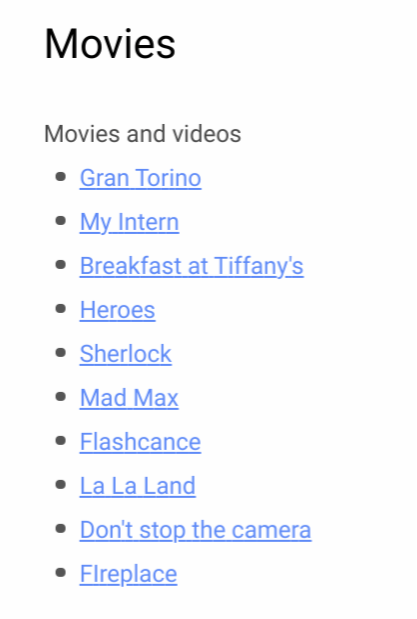
\includegraphics[width=40mm,bb=0 0 417 619]{figures/2690db244045aa809a3e2fc2b40ba0a3.png}}
\centerline{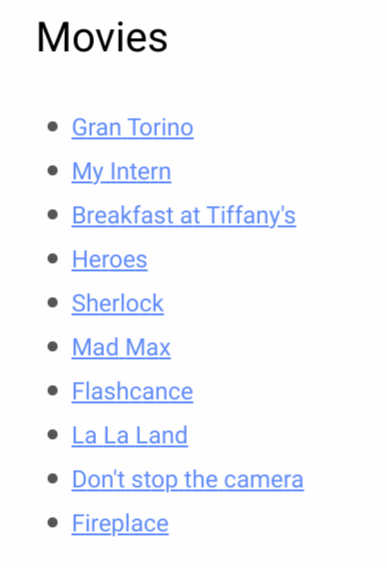
\includegraphics[width=40mm,bb=0 0 387 568]{figures/2b97930bf5730fcaf4d9c0adeb9c5f6e.png}}
\caption{Movie list.}
\label{movielist}
\end{figure}

The raw text of this page is shown below:

{\scriptsize
\begin{verbatim}
Movies
 [https://www.netflix.com/watch/70105600 Gran Torino]
 [https://www.netflix.com/watch/80047616 My Intern]
 [https://www.netflix.com/watch/330201 Breakfast at Tiffany's]
 [https://www.netflix.com/watch/70080178 Heroes]
 [https://www.netflix.com/watch/70174781 Sherlock]
 [https://www.happyon.jp/watch/100048550 Mad Max]
 [https://www.netflix.com/watch/60010351 Flashcance]
 [https://www.netflix.com/watch/80095365 La La Land]
 [https://www.netflix.com/watch/81191988 Don't stop the camera]
 [https://youtube.com/embed/AtZr9g2vwrI?autoplay=1 Fireplace]
\end{verbatim}}

\begin{figure}[H]
% \centerline{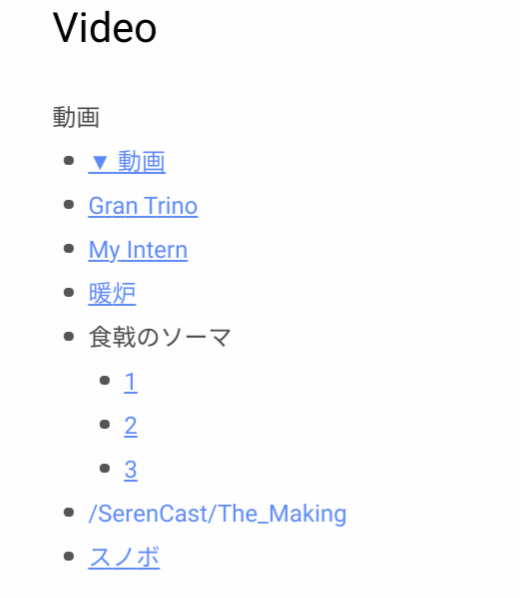
\includegraphics[width=80mm,bb=0 0 524 598]{figures/65b01a87b67c9a8e838a047b945f6a77.png}}
\centerline{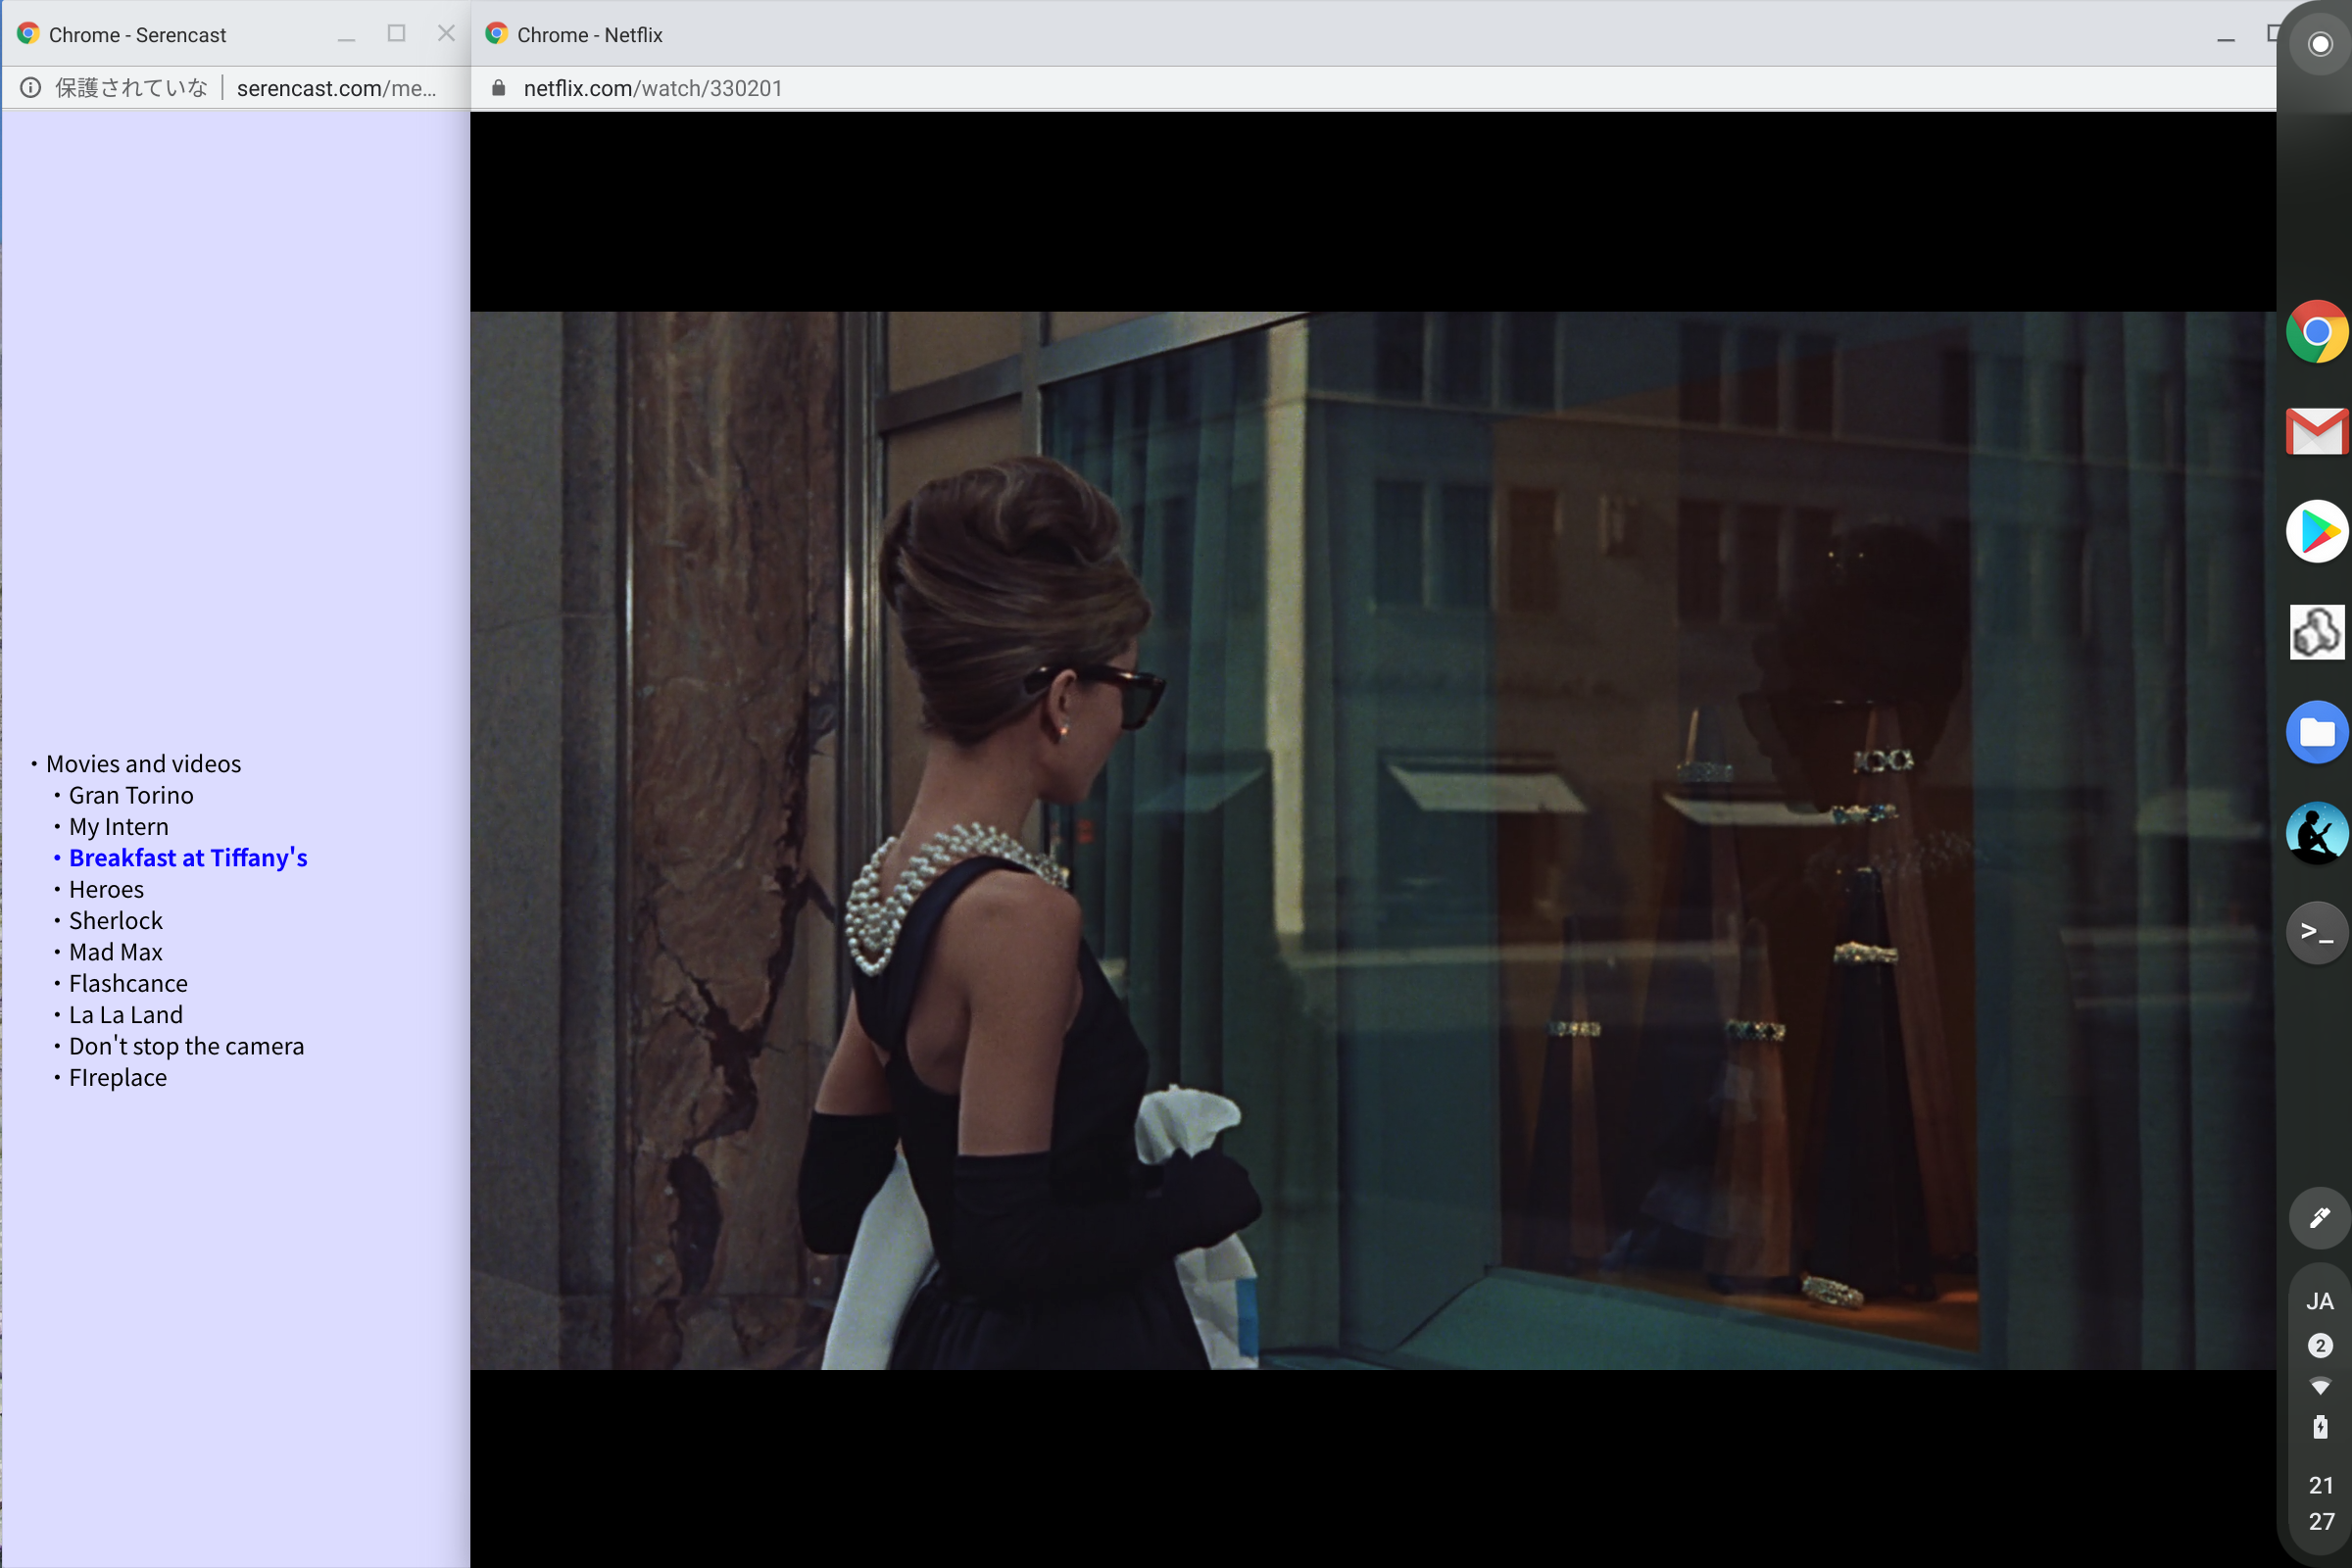
\includegraphics[width=80mm,bb=0 0 2400 1600]{figures/e8ae562a5a68a1955ac70b4faed9a146.png}}
\caption{Showing a movie.}
\label{tiffany}
\end{figure}

When we access the {\SB} page from {\SC},
``Gran Trino'' from Netflix automatically starts in the right side of the screen,
just like a TV program starts when we rotate tha channel dial of an old television.
When the user pushes the {\down} key twice,
``Breakfast at Tiffarny's'' is selected and
the movie starts at the right side of the screen. (Figure \ref{tiffany})

In the above example, we can select only one of the 10 movies using the Gear interface.
But we can add more data by hierarchically providing more contents in {\SB} pages.

In one page, we can specify a hierarchical structure by using indentations.
Figure \ref{musiclist} shows a portion of a list of CDs and
musics titles by ``Weather Report'' and ``Wes Montgomery'' are shown\footnote{
  Weather Report is the name of a famous Jazz group, and Wes Montgomery is a famous Jazz guitarist.
}.
For example, 
``Black Market'' is the first title in the album ``8:30'' of ``Weather Report'', and
``Scarlet Woman'' follows ``Black Market''.
``Wes Montgomery'' is listed in the same layer as ``Weather Report'', and
the album ``Tequilla'' is listed one level below the level of the name of the artist.

\begin{figure}[H]
% \centerline{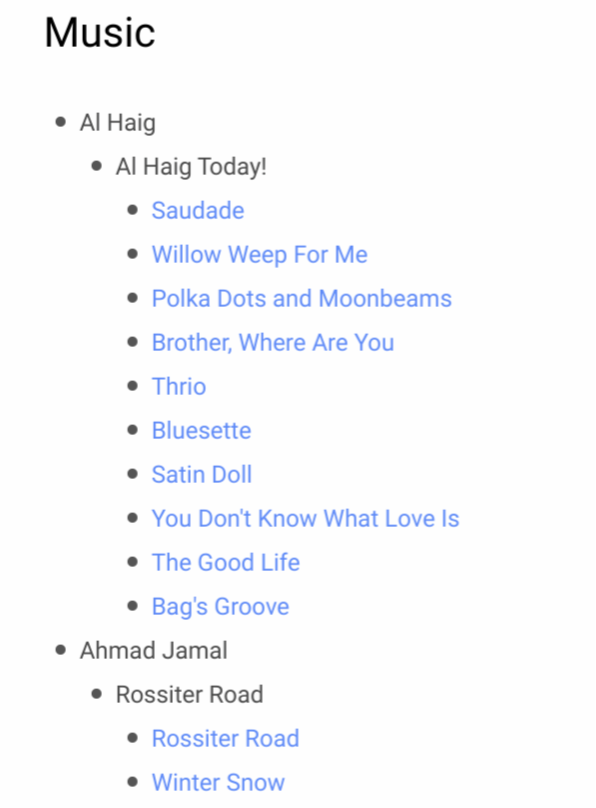
\includegraphics[width=40mm,bb=0 0 596 808]{figures/6657544cf60cbf0aea91ba7da0455b90.png}}
\centerline{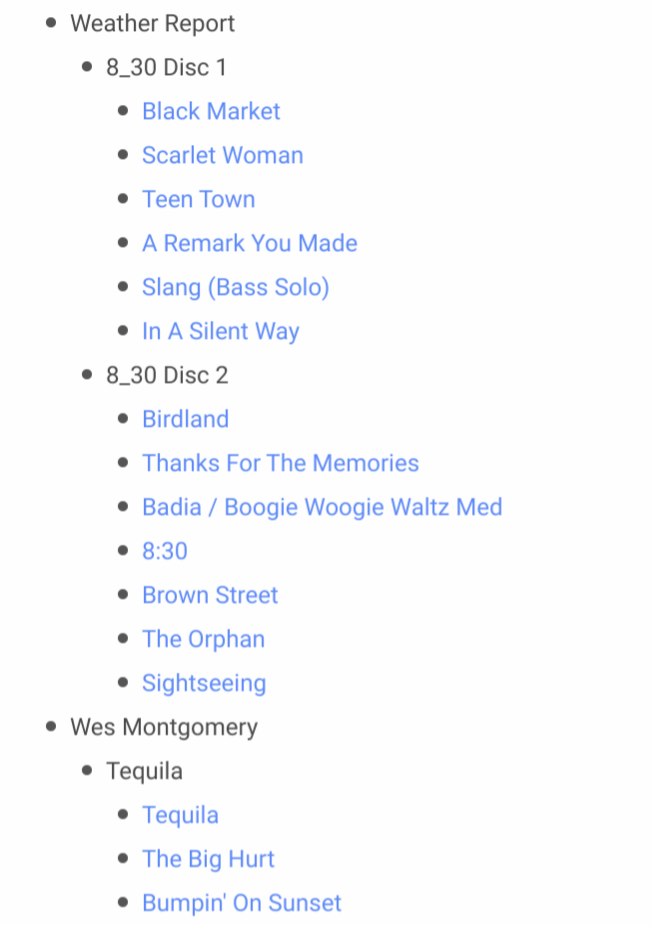
\includegraphics[width=40mm,bb=0 0 652 926]{figures/d8fe8ff8f3e1bbcb34cf51e268592f8c.png}}
\caption{Music list.}
\label{musiclist}
\end{figure}

The title of this {\SB} page is ``Music'', and 
we can collect Movie page, Music page, and other pages by
listing them in another page (``Top'' page, in this case).

\begin{figure}[H]
\centerline{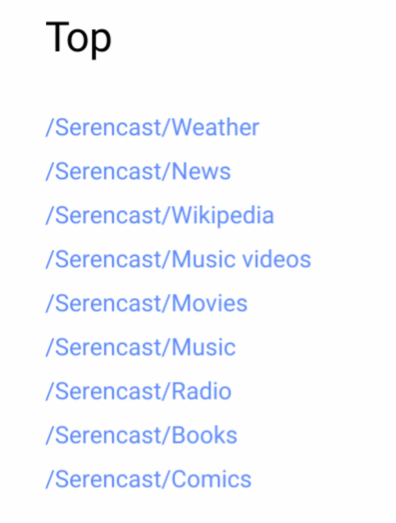
\includegraphics[width=40mm,bb=0 0 396 523]{figures/8a8e4d63b75183f1b4d0ed4db733f500.png}}
\caption{Top page.}
\label{top}
\end{figure}

Many pages (Music, Movies, etc.) are listed in the Top page, and
the pages are treated as children pages of the Top page.
By constructing data hierarchically like this,
We can build a very large hierarchical database for watching movies, videos, news, etc.
A hierarchical database with
As many as 100,000 pages can be easily constructed on a {\SB} pages, and
we can select one of the entries only by using only {\up} and {\down} keys,
using the Gear technique described in section \ref{navigation}.

\begin{figure}[H]
\centerline{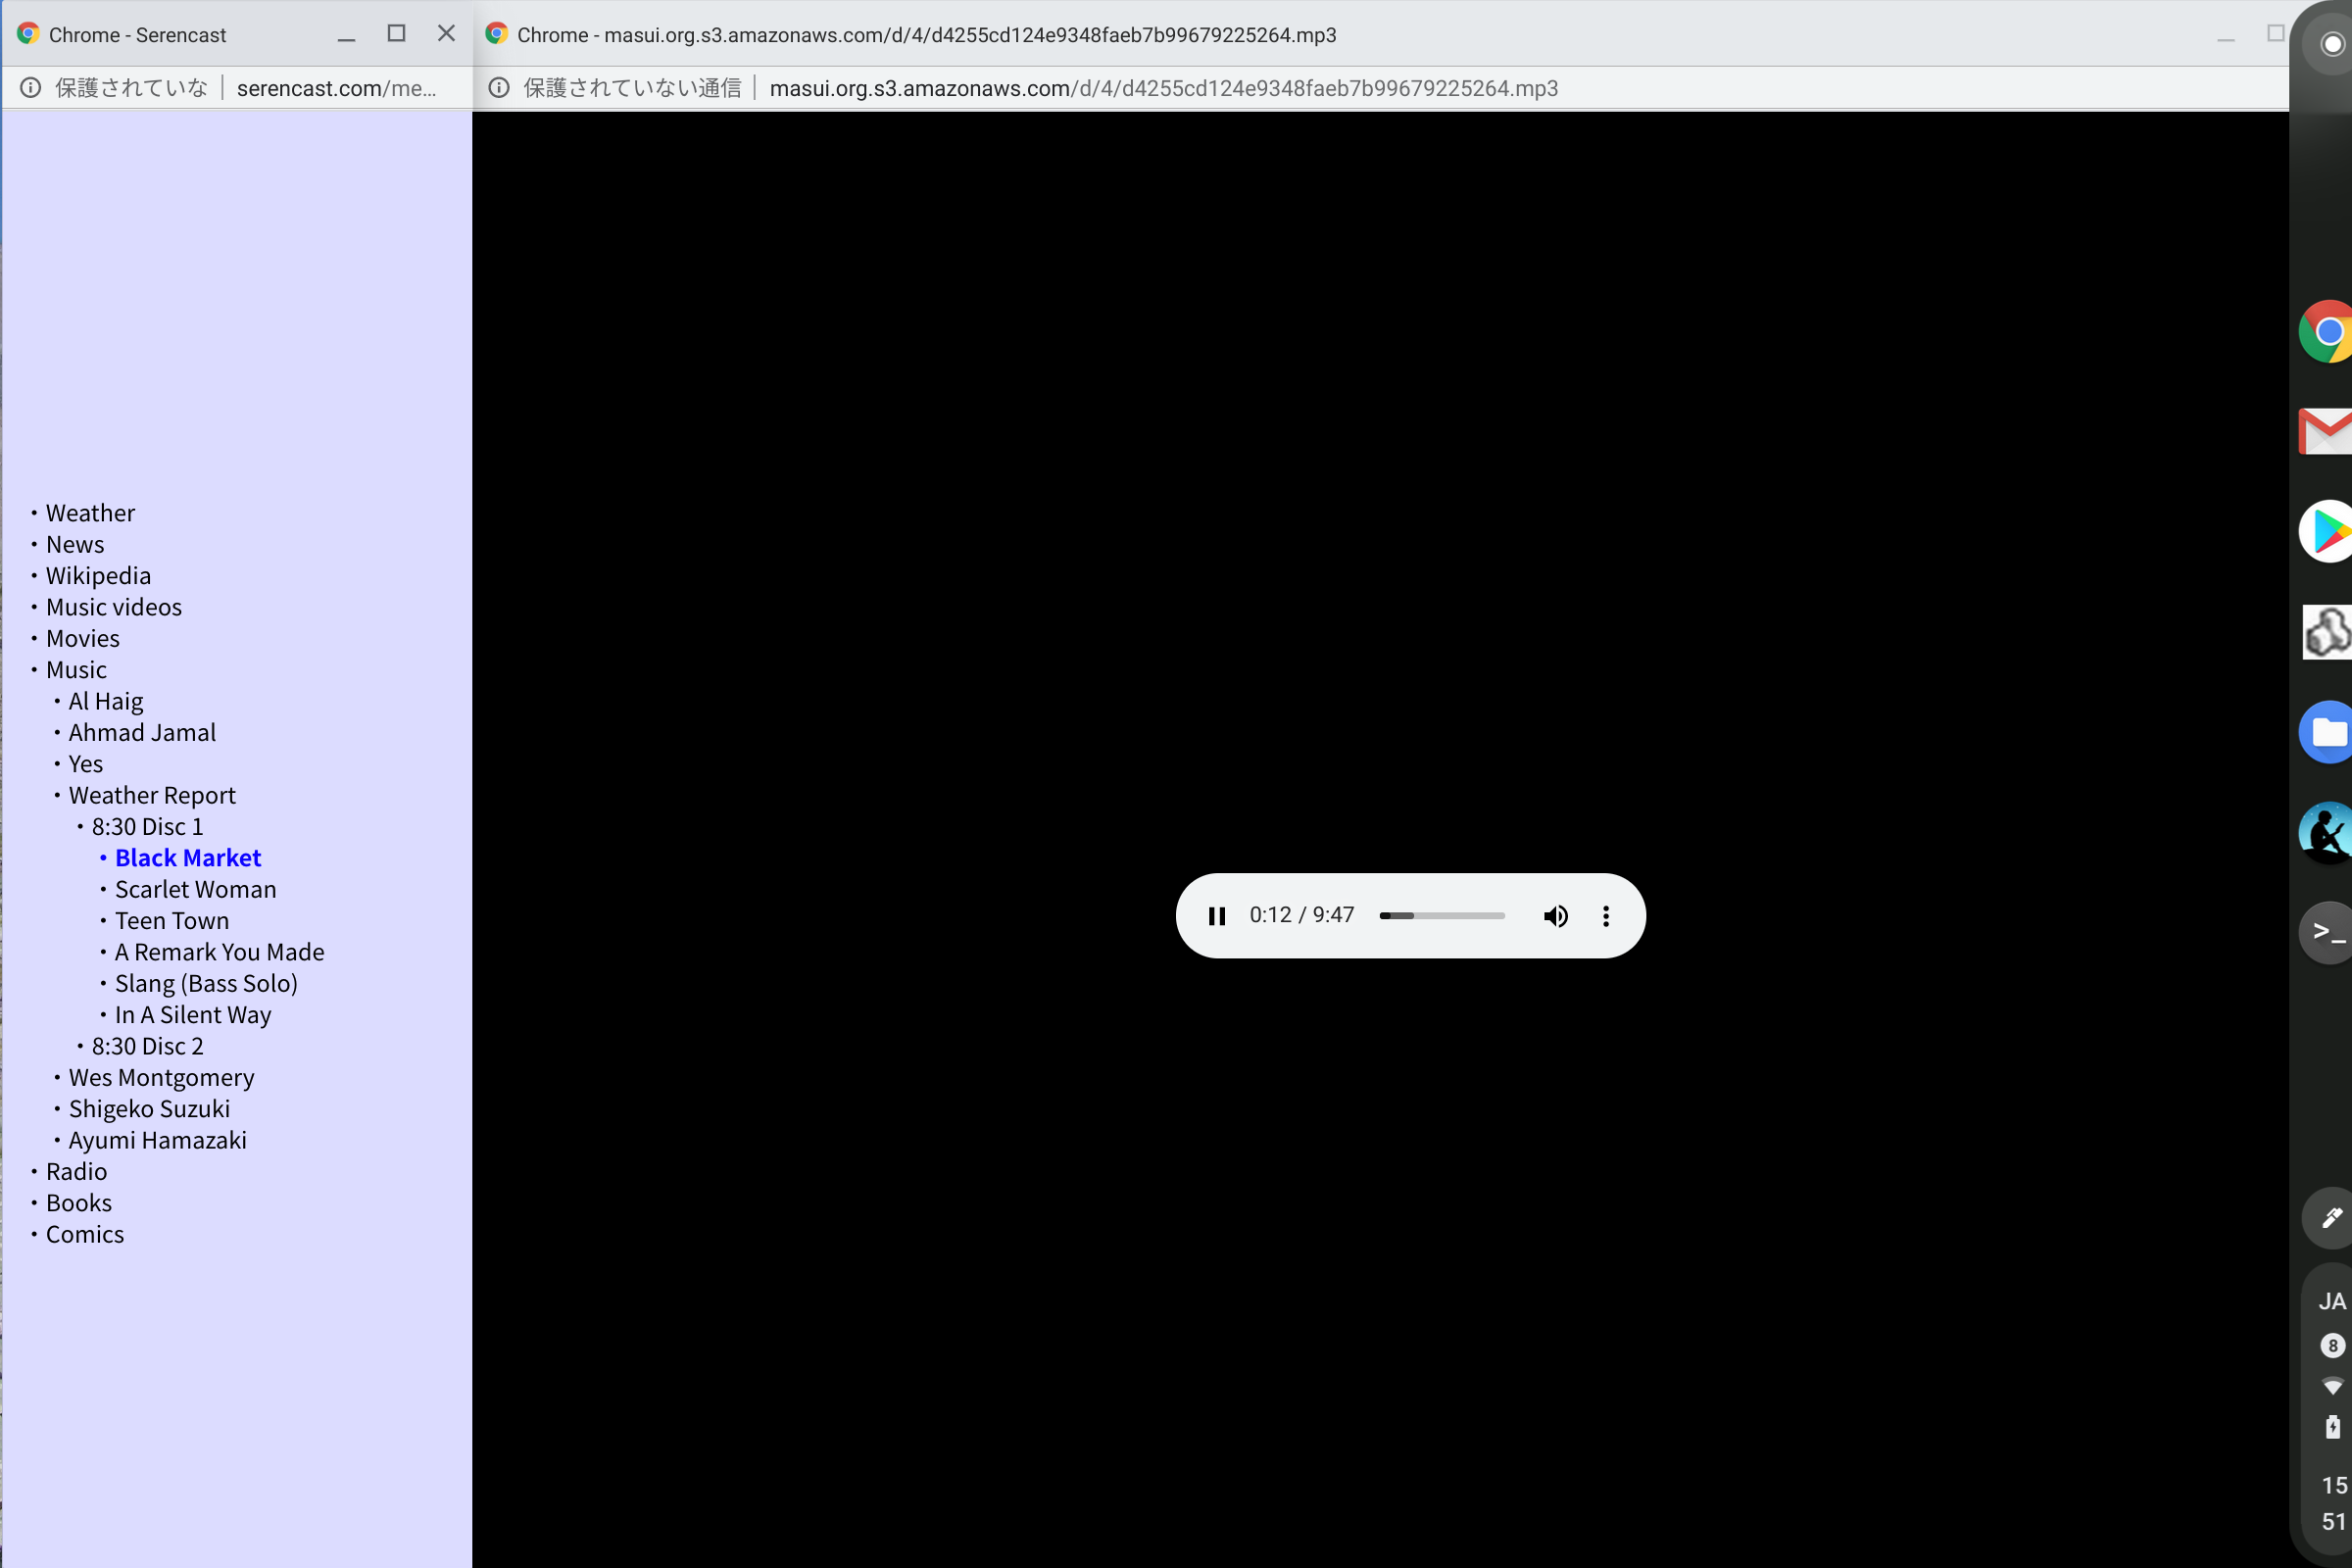
\includegraphics[width=80mm,bb=0 0 2400 1600]{figures/blackmarket.png}}
\caption{Playing a music.}
\label{blackmarket}
\end{figure}

\begin{figure}[H]
\centerline{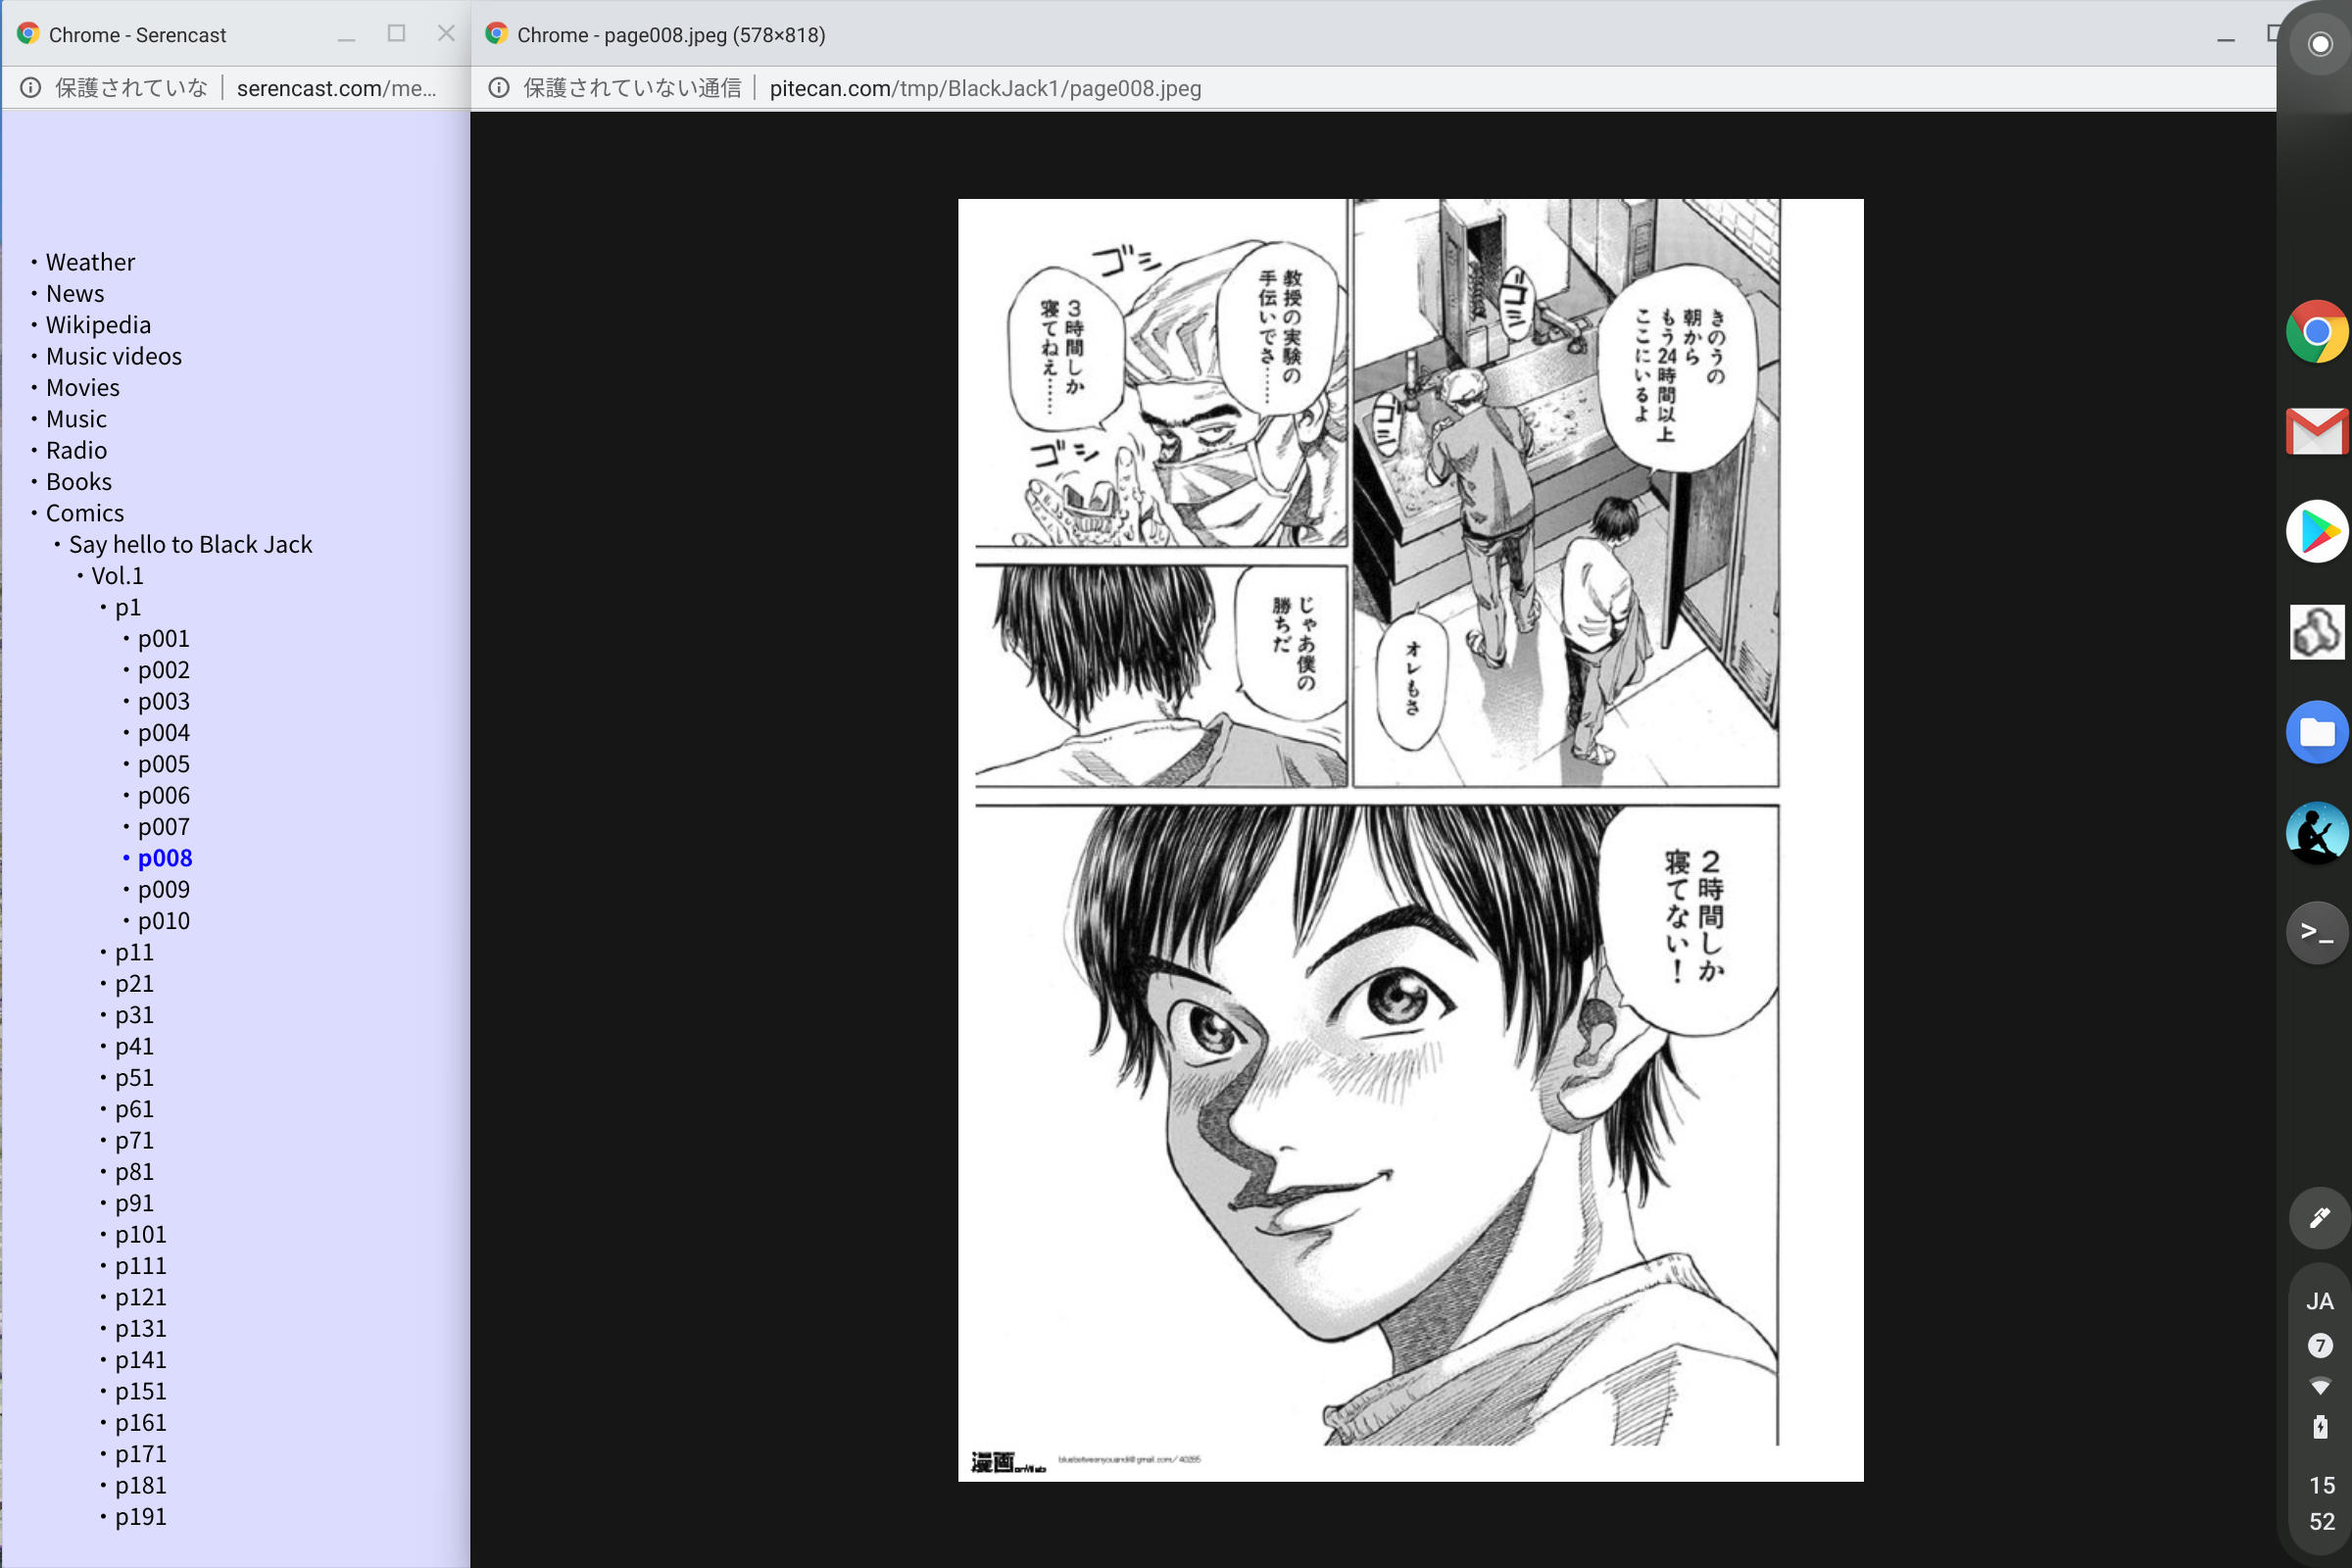
\includegraphics[width=80mm,bb=0 0 2400 1600]{figures/blackjack.png}}
\caption{Reading a comicbook.}
\label{blackjack}
\end{figure}

Since anybody can edit the {\SB} page and construct the hierarchical data,
people can enjoy creating their own data by editing their {\SB} pages.
Also, when people who want to advertise their works,
they can create their {\SB} page
and give it to others so that other people can include the page
in their list and enjoy it using Gear.

\section{DISCUSSIONS}

\subsection{Input devices for Gear}

Since only two switches are required in the Gear interface,
various kinds of input devices can be used for Gear.
We have tried various input devices, and collected experiences.

\paragraph{Keys and buttons}

The simplest input device for Gear may be keyboards or buttons.
We tried using arrow keys on a PC, and it works fairly fine.
We also tried special devices with pressure sensors, with which users can press the button strongly to simulate multiple keyboard presses.
Two keys or pressure sensors can be placed anywhere: we tried putting two pressure sensors at the bottom of a chair, and it worked fine.

We can use two arrow keys on a computer keyboard for using {\SC}.
It works fine, but Gear is not more useful than using many keys on a computer.
%
Good thing is that many keyboard devices are available for personal computers,
and we can use such devices for using Gear.
``Key-repeat'' feature is useful for fast scrolling of the menu.

\paragraph{Rotating devices}

We tried various rotating devices for Gear.
Many kinds of rotating input devices have been used for controlling TVs and VCRs so far.
For example, ``jog dials''ave been widely used for controlling VCRs, and we tried the device for Gear.

(figure)

We have also tried "rollers" for Gear.
After trying these devices, we found that controlling rotating devices are not as easy as we expect,
because presice control of a hand is fairly difficult.
People are good at controling fingers, but people are usually not very good at controlling hands.

We also tried mouse wheels, and found that mouse wheels are very suitable for using Gear, because
we are good at presice control of our fingers.


We can use a rotary encoder as a 

\begin{figure}[H]
\centerline{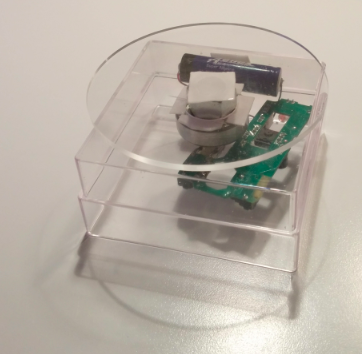
\includegraphics[width=54mm,bb=0 0 362 354]{figures/ff2d18e66f9a4655dbb5e22e0bb9a0ae.png}}
\caption{A disk-based device for Gear.}
\label{disk}
\end{figure}

We used
PowerMate\footnote{
  \textsf{http://griffintechnology.com/support/powermate}
} from Griffin Technology for the rotating device.
PowerMate generates standard keyboard events when rotated,
and no special programming techniques are required.
%
Users can explore all the contents just by
rotating the device clockwise and counterclockwise.

\begin{figure}[H]
\centerline{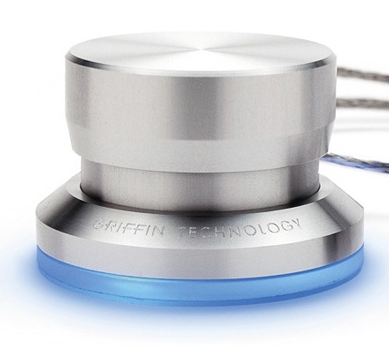
\includegraphics[width=30mm,bb=0 0 389 348]{figures/d3a69499f7e7314ae6dc10f5bf3a2be5.png}}
\caption{A PowerMate used for the prototype.}
\label{powermate}
\end{figure}

\paragraph{2-way lever}

We have also tried to use a paddle-like device for generating {\U} and {\D}.
Users can push the puddle to the right to generate {\U} and
left to generate {\D}.
Pressure sensors are installed on the puddle, and
many {\U}s are generated when the user pushs the puddle strongly.

\begin{figure}[H]
  \centerline{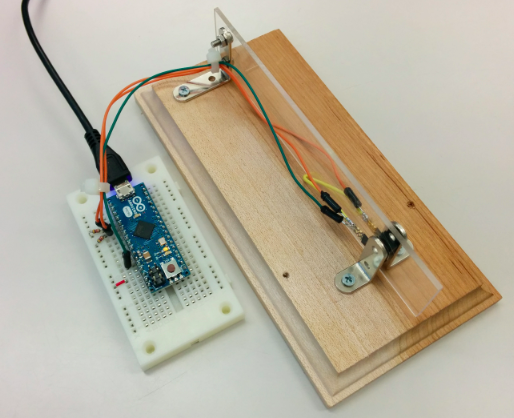
\includegraphics[width=54mm,bb=0 0 514 418]{figures/3c2de63899653056f3c6be835b9aaf43.png}}
\caption{Paddle device for Gear.}
\label{paddle}
\end{figure}

Controling the speed of the scrolling of Gear by pressure is convenient,
since sometimes users want to jump to a far entry from current position.
That behavior is close to the key-repeat feature or computer keyboards.

\comment{
We tried a lever with two pressure sensors.
モールス用「エレキー」
Puddle

\begin{figure}[H]
\centerline{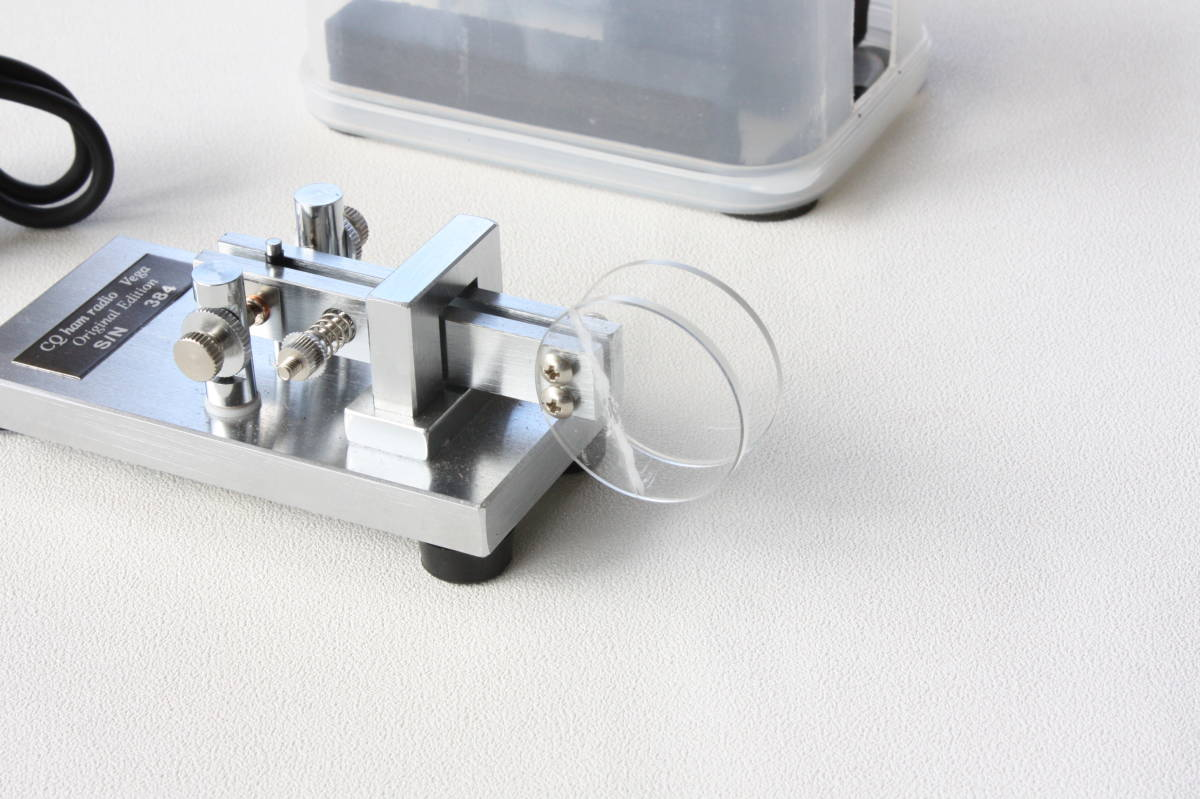
\includegraphics[width=80mm,bb=0 0 1200 799]{figures/d64d2a8e1dddc57f693267f811510f23.jpg}}
\caption{Elekey.}
\label{elekey}
\end{figure}

}


After trying various devices, it became clear that simple buttons or
wheels can be put at anywhere like on the table or under a chair, and
we felt that the integration of furniture and input devices will be
important in the IoT age.

If we can put input devices that fits to furnituers, we can use the device near the furniture, without making the input devices look awkward.
  入力装置つきのカッコ良い家具が作れる
 If we can put the devices neatlly on furnitures and beds, people with disabilities can easilyt use them, 
 体が不自由でも使えることは間違いない

\comment{
\section*{IMPLEMENTATION}

A large list of news articles, movies, anime films, musics, and e-book titles are listed in one browser window
and the content is displayed in another window (Figure \ref{screenshot}).

\begin{figure}[H]
\centerline{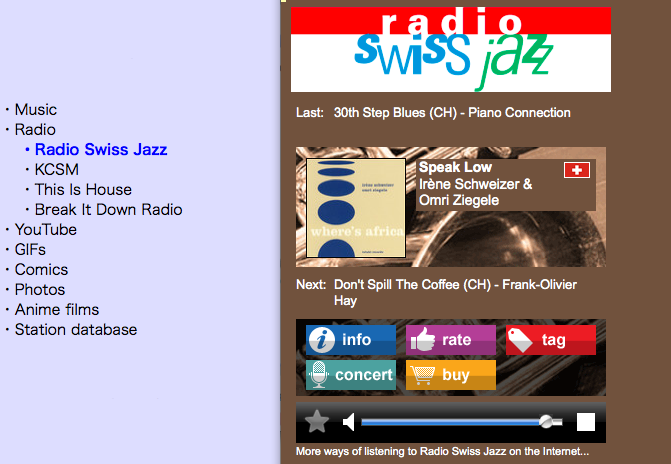
\includegraphics[width=80mm,bb=0 0 671 464]{figures/95cf2fec71c52ead6fdbcb7f79aca654.png}}
\caption{Selecting an Internet radio station.}
\label{screenshot}
\end{figure}
}

\section*{DISCUSSIONS}

\subsection{Comparison with existing navigation methods}

4-way navigation is commonly used for exploring hierarchical data structure,
and it is familiar to computer users.
Some mobile phones and PDAs are equipped with a jog dial with a push button,
where the dial is used for choosing an item from the list and 
the push button is used for fixing the selection.
% PowerMate is equipped with a push button which can used for such purposes.
% As far as we know,
All the existing methods require more than 2 keys/buttons, and
to the best of the authors' knowledge,
Gear is the only interaction method for exploring hierarchical data structure
with one rotating device.

Using a conventional hierarchical menu,
child elements are displayed automatically when their parent element is selected by a mouse.
The behavior is well understood by computer users,
and Gear's automatic transition (e.g. from Figure \ref{fig4} to Figure \ref{fig5})
looks familiar to users.

\subsection{Comparison with InfoVis techniques}

Various information visualization techniques like
Treemap\cite{Johnson:1991:TSA:949607.949654},
Hyperbolic Tree\cite{Lamping:1995:FTB:223904.223956},
and Sunburst\cite{Stasko:2000:FDN:857190.857683}
have been proposed for visualizing large hierarchical data.
Zooming user interface (ZUI) systems like
Pad\cite{Perlin:1993:PAA:166117.166125} and
Pad++\cite{Bederson:1994:PZG:192426.192435}
can also be used for handling large hierarchical data laid out in a 2D space.
%
These visualization techniques and descendent technologies have become popular these days and
all of these systems are useful for understanding the structure of
large hierarchical data, but users of these systems have to use a pointing device
to take full advantage of their advantages.

% More conventional visualization techniques like TreeView\footnote{
%   \textsf{http://en.wikipedia.org/wiki/Tree\_view}
% } by replacing 4-way navigation to our approach.

% {\ST} can be adopted to more conventional visualization techniques like
% TreeView\footnote{
%   \textsf{http://en.wikipedia.org/wiki/Tree\_view}
% } by replacing 4-way navigation to our approach.

It seems to be a good idea to use Gear on more conventional visualization techniques like
TreeView\footnote{
  \textsf{http://en.wikipedia.org/wiki/Tree\_view}
}, by replacing 4-way navigation to Gear.

% LensBar\cite{Masui:1998:LVB:647341.721215}
% is also a ZUI system for handling large hierarchical data,
% but the same data structure used in LensBar can be used for Gear.
% Users can use a pointing devices when it is appropriate,
% and use two keys or a disk device when pointing devices is not available.

\subsection{Timing control}

The biggest disadvantage of Gear is that
the behavior of Gear depends on the speed of the user's operations.
In Figure \ref{fig4},
if a user wanted to select \tsf{Clothing} but couldn't issue {\down}
quickly enough, he will see Figure \ref{fig5} instead of Figure \ref{fig7}.
This is a tradeoff between usability and simplicity, and
the best parameter should be set based on the user and the Gear device.

\section{Discussions}

\subsection{Is the Gear interface a new idea?}
  Since the idea of Gear interface is so simple, we have been wondering if the same idea had been around in the past.
  But as far as we know, Gear is the first attempt to explore 

 こういうデバイスは超簡単なので、存在した可能性はある
 特許や論文を調べた限りはみつけられなかった

\section*{EVALUATION}

\begin{verbatim}
実際に家で使っていた
 階層構成の問題点はあるが、いろんな階層を用意しておけばいい
  時間的階層、アーティスト的階層、名前的階層、...
  それはなんとか対応できることをいう
   もちろん同時に指定できればいいのだが...
 音量とか場所とかは?
 名前があるものは必ず階層的に検索できる
  e.g. 辞書
\end{verbatim}

No formal evaluation have been done yet, but Gear has been used in the author's
living room for six months, and the author's family members are using it
everyday for watching anime films and listening to music.
Besides PowerMate, a wireless mouse is also used,
since we can carry it anywhere and select
a film or a music just by rotating the mouse wheel.

We demonstrated Gear at an exhibition
held in November 2013, and asked more than 100 people to try it
(Figure \ref{exhibition}).
%
Since the only thing a user can do with Gear is to rotate the device,
users seemed to be able to understand the behavior of Gear with trials and errors.
% 
% a user can use the device and see what happens without thinking about
% other interactions.
% 
Using only one rotating device for data navigation is a new experience for
all the subjects, but the hard restriction of the device seemed to have worked in this case.

\begin{figure}[H]
\centerline{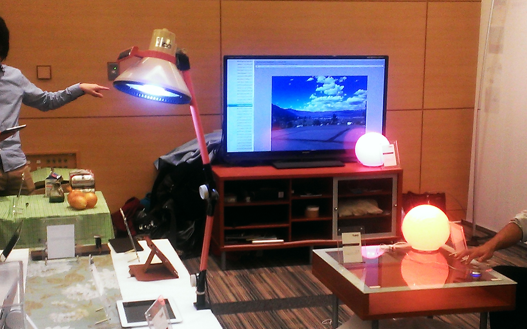
\includegraphics[width=70mm,bb=0 0 527 329]{figures/c520d5dfbd06c532d48d324a7019b00c.png}}
\caption{People at the right using {\SC} at an exhibition.}
\label{exhibition}
\end{figure}

% Selecting a content only by rotating a dial is very 気持ち良い。
% 音楽ソース、ニュースソース、動画、Wikipediaなどあらゆるものをダイヤルやペダルだけで検索できる

\section*{CONCLUSIONS}

We have developed a new simple interaction method ``Gear'' for exploring
large hierarchical data structure.
A Gear user can easily find an entry in a huge hierarchical database
only by using a rotating input device which can be installed at
wide range of locations where conventional keyboards and switches do not fit.
We are hoping to install various implementations of Gear and try them at
various places like kitchens, restrooms, etc.

\small{
\bibliographystyle{plain}
\bibliography{paper}
}

\end{document}

Non-click browsingの威力
  ストレスが全然違う
音声を使う
満員電車で使える
速度
  log(n)
時計のセットとか




